\section[部分动态布局]{部分动态布局}
Android中的动态布局指的是ListView等物理尺寸跟显示尺寸不一致的布局,
而“部分”动态布局指的是一个布局中既有固定的布局,如一个button,又有
动态布局,如一个ListView。

动态布局可以灵活的设置显示尺寸,但是我们
并不想固定住它的显示尺寸,比如一个可旋转的dialog,实际内容介于屏幕
宽度和高度之间,于是我们要求横屏时高度占满屏幕,而竖屏时根据内容自动
设置高度,因为竖屏时如果高度也占满屏幕的话就有有空白,影响美观效果。

下面是一种实现方式,

\begin{xmlcode}
<?xml version="1.0" encoding="utf-8"?>
<LinearLayout
  xmlns:android="http://schemas.android.com/apk/res/android"
  android:layout_width="320dp"
  android:layout_height="wrap_content"
  android:orientation="vertical">
  <TextView
    android:id="@+id/rotate_dialog_title"
    android:layout_width="match_parent"
    android:layout_height="wrap_content"
    android:layout_weight="0"
    android:text="This is title"/>
    
  <ListView
    android:id="@+id/rotate_dialog_content"
    android:layout_width="match_parent"
    android:layout_height="wrap_content"
    android:layout_weight="1"/>

  <Button
    android:id="@+id/rotate_dialog_button"
    android:layout_width="match_parent"
    android:layout_height="wrap_content"
    android:layout_weight="0"
    android:text="This is OK button"/>
</LinearLayout>
\end{xmlcode}

其中的layout\_weight起关键作用,如果没有此属性,当ListView的
内容很长而超过屏幕高度(宽度,横屏下)时,底部的button就被挤没了,
因为LinearLayout默认按照顺序排列,先到先得,如果没有空间的话
后面的控件就消失了。

在这种实现中,中间部分即是不是动态布局也无妨,比如中间放一个大大
的text view,只是中间的布局显示不全而已,见图 \ref{fig:dynamic}。
\begin{figure}[ht]
  \centering
  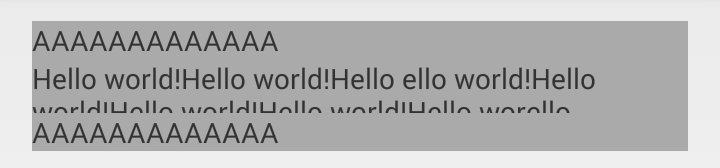
\includegraphics[width=.7\textwidth]{picturedir/dynamic_layout.png}\\
  \caption{Life cycle of Service}\label{fig:dynamic}
\end{figure}
